\documentclass[10pt,twocolumn,letterpaper]{article}
\usepackage[T1]{fontenc}
\ifdefined\reviewcopy
\usepackage[review]{cvpr}
\else
\usepackage[pagenumbers]{cvpr}
\fi
\usepackage{microtype}
\usepackage[pagebackref,breaklinks,colorlinks,allcolors=blue]{hyperref}
\def\paperID{0000}
\def\confName{CVPR}
\def\confYear{2026}
\newcommand{\EpisodeCount}{1,421}
\newcommand{\ProbeCount}{7,020}
\newcommand{\PairCount}{308}
\newcommand{\QuestionCount}{8,441}
\newcommand{\SourceCount}{97}
\newcommand{\ProfileCount}{412}
\newcommand{\OracleCount}{650}
\newcommand{\BaseProfileCount}{98}
\newcommand{\ContextProfileCount}{314}
\newcommand{\ZeroYieldProfileCount}{270}
\newcommand{\NewSourceCount}{81}
\newcommand{\CandidateCount}{100}
\newcommand{\AdmittedCount}{81}
\newcommand{\RejectedCount}{19}
\newcommand{\NewSampledEpisodeCount}{972}
\newcommand{\GoalsPerSource}{2}
\newcommand{\JobSettingsPerSource}{3}
\newcommand{\StartsPerMission}{2}
\newcommand{\EpisodesPerNewSource}{12}
\newcommand{\PrimaryPairCount}{36}
\newcommand{\PrimarySourceCount}{12}
\newcommand{\PrimaryInterventionCount}{18}
\newcommand{\PrimaryStartCount}{36}
\newcommand{\HistoricalPairCount}{10}
\newcommand{\QualifiedInterventionCount}{116}
\newcommand{\ZeroYieldInterventionCount}{98}
\newcommand{\ContextSubsetCount}{230,138}
\newcommand{\MatchedOptionCount}{1,911}
\newcommand{\ProductCount}{61,093,730}
\newcommand{\EdgeCount}{757,651,278}
\newcommand{\MaxGap}{18}
\newcommand{\OldLabels}{1,802,728}
\newcommand{\CalibrationCount}{50}
\newcommand{\DiscriminativeCount}{6,970}
\newcommand{\ProblemCount}{6,830}
\newcommand{\RepeatedRowCount}{190}
\newcommand{\NextActionCount}{2,595}
\newcommand{\ContinuationCount}{432}
\newcommand{\GeometryQuestionCount}{92}
\newcommand{\AppearanceQuestionCount}{72}
\newcommand{\RepairCount}{3,829}
\newcommand{\SequencePairCount}{216}
\newcommand{\AppearancePairCount}{36}
\newcommand{\SequencePairsPerBin}{72}
\newcommand{\RepairMin}{1}
\newcommand{\RepairMax}{13}
\newcommand{\InverseCorrect}{2,260}
\newcommand{\InverseSuboptimal}{1,487}
\newcommand{\InverseUnavailable}{82}
\newcommand{\DepthOneContainsOptimal}{2,595}
\newcommand{\MeshCount}{449}
\newcommand{\TriangleCount}{523,571}
\newcommand{\PolicyRuns}{4,263}
\newcommand{\RawPolicyRuns}{39,788}
\newcommand{\DevelopmentEpisodeCount}{445}
\newcommand{\DevelopmentSourceCount}{34}
\newcommand{\DevelopmentPrimaryPairCount}{12}
\newcommand{\DevelopmentPrimarySourceCount}{3}
\newcommand{\HeldoutEpisodeCount}{976}
\newcommand{\HeldoutSourceCount}{63}
\newcommand{\HeldoutPrimaryPairCount}{24}
\newcommand{\HeldoutPrimarySourceCount}{9}
\newcommand{\GreedyCompleted}{4,163}
\newcommand{\GreedyAssigned}{4,263}
\newcommand{\GreedyOptimal}{3,642}
\newcommand{\GreedyMaxExpansions}{0}
\newcommand{\GreedyMedianExpansions}{0}
\newcommand{\DispatchCompleted}{4,132}
\newcommand{\DispatchAssigned}{4,263}
\newcommand{\DispatchOptimal}{3,642}
\newcommand{\DispatchMaxExpansions}{0}
\newcommand{\DispatchMedianExpansions}{0}
\newcommand{\BoundedSmallCompleted}{4,075}
\newcommand{\BoundedSmallAssigned}{4,263}
\newcommand{\BoundedSmallOptimal}{4,075}
\newcommand{\BoundedSmallMaxExpansions}{100}
\newcommand{\BoundedSmallMedianExpansions}{13}
\newcommand{\BoundedLargeCompleted}{4,199}
\newcommand{\BoundedLargeAssigned}{4,263}
\newcommand{\BoundedLargeOptimal}{4,199}
\newcommand{\BoundedLargeMaxExpansions}{1,000}
\newcommand{\BoundedLargeMedianExpansions}{13}
\newcommand{\FullSearchCompleted}{4,263}
\newcommand{\FullSearchAssigned}{4,263}
\newcommand{\FullSearchOptimal}{4,263}
\newcommand{\FullSearchMaxExpansions}{14,307}
\newcommand{\FullSearchMedianExpansions}{13}
\newcommand{\InverseAccuracy}{59.0\%}
\newcommand{\DepthOneUniform}{97.4\%}
\newcommand{\UniformCandidateAccuracy}{32.6\%}
\newcommand{\PrefixZeroAccuracy}{50.0\%}
\newcommand{\PrefixTwoCorrect}{234}
\newcommand{\PrefixTwoTotal}{432}
\newcommand{\PrefixFiveCorrect}{288}
\newcommand{\PrefixFiveTotal}{432}

\newcommand{\ResourceCaseCaption}{Exact oracle replay of \texttt{roadster-\allowbreak{}body-\allowbreak{}05} from source 31027. The displayed operations are 0, 14, 28, 42; the certified optimum is 42 operations. This is a software witness, not a model trajectory.}
\newcommand{\GeometryCaseCaption}{Primary inventory-matched pair \texttt{source-\allowbreak{}v23-\allowbreak{}10037-\allowbreak{}matched-\allowbreak{}0/\allowbreak{}geometry/\allowbreak{}future-\allowbreak{}00} from held-out source 10037 in the initial isometric view. Both contexts use 63 source pieces (47 fixed); the exact part-number/color multiset, registered poses, start, target, rack, work, and plan match. After 2 shared legal operations, the exact labels are context 1: first conflict at operation 3; context 2: all legal. Only subsets of original fixed instances change. These publication views omit ID overlays; answers are evaluator annotations. Pixel distinction is not perceptual answerability.}
\newcommand{\RepairCaseCaption}{Certified lag-5 repair, \texttt{source-\allowbreak{}10036-\allowbreak{}35/\allowbreak{}repair-\allowbreak{}lag-\allowbreak{}5}, source 10036. A: the pre-error checkpoint defines the optimal corridor. B: an error and 5 further operations leave it. The last history action is \texttt{attach P013}. Undoing it first requires 9 operations to repair; the optimum takes 7, starting with \texttt{detach P002}. C: a nonterminal corridor state is restored. These are oracle replay frames, not model reasoning or a model success; exact source instances and actions are archived.}

\title{BrickPlan: Diagnosing Future Action Cost and Error Recovery\\in Visual Assembly Planning}
\author{Benchmark research release 2.3\\Population model and human studies pending}
\begin{document}
\raggedbottom
\maketitle

\begin{abstract}
Visual assembly planning requires predicting how an action changes later
access, workspace occupancy, and unfinished work. Final-shape accuracy
alone does not isolate these abilities. We introduce BrickPlan, an
executable benchmark with exact future-cost and recovery labels under
a finite assembly abstraction. Original LDraw geometry determines
qualified motions and connectivity; a limited rack and persistent
off-assembly inspection ledger couple decisions over time.
The release contains \EpisodeCount{} interactive episodes and
\ProbeCount{} diagnostic questions from \SourceCount{} source groups.
Matched sequences test future legality, inventory-matched fixed contexts
test geometric dependence, and delayed-repair questions exclude the goal from
recovery credit. Static diagnostics supply four fixed views; active
diagnostics charge additional acquisitions. Calibration questions and
repeated variants receive explicit scoring treatment.
The primary geometry cohort contains \PrimaryPairCount{} pairs from
\PrimarySourceCount{} sources, with both exact conflict labels required.
Structural controls reveal scope and limits: closure greedy completes
\GreedyCompleted{} of \GreedyAssigned{} task-runs, \GreedyOptimal{} optimally;
an inverse-last-action control solves \InverseAccuracy{} of recovery
questions. We release native-resolution
observations, exact evaluators, a question workbench, and a preserved
historical model trace. These measurements characterize the instrument;
population visual-model and human performance remain unmeasured.
\end{abstract}

\section{Introduction}
An assembly action can be legal now and expensive later. Removing a
piece may consume the last available holder before a deeper part becomes
accessible; replacing another may obstruct unfinished inspection work.
If an agent detects an error after several further actions, reversing
its latest action need not restore an efficient completion.
Measuring these effects requires more than recognizing brick types
or comparing a final image.

BrickPlan asks whether an agent can predict the \emph{future action cost}
of a visible assembly decision and recover after a costly choice has
propagated. We distinguish immediate rejection, a legal action that
increases exact remaining cost, and failure to return to an optimal
completion corridor. Restricting placements to registered original
sites makes these distinctions exhaustively labelable. This deliberate
restriction trades manipulation breadth for exact diagnostic targets.

A preceding assembly-only bank illustrates the need for explicit
controls. An occupied-blocker closure formula reproduced all
\OldLabels{} stored state--goal costs. Long solutions alone did not
establish deep planning. BrickPlan adds finite external storage and
inspection work whose completion persists after reattachment. Static
relations remain useful, but occupancy alone no longer specifies the
mission state or exact cost.

Our contributions are threefold. First, we define an executable visual
assembly task with resource and work obligations, interactive episodes,
and explicit checkpoint diagnostics. Second, we construct sequence,
geometry, appearance, and recovery controls, with separate static and
active observations and auditable scoring units. Third, we release
the construction, execution, evaluation, and publication pipeline,
including strong structural controls. We do not infer a human--model
gap, required internal reasoning depth, or broad physical competence
from software verification.

\begin{figure*}[t]
\centering
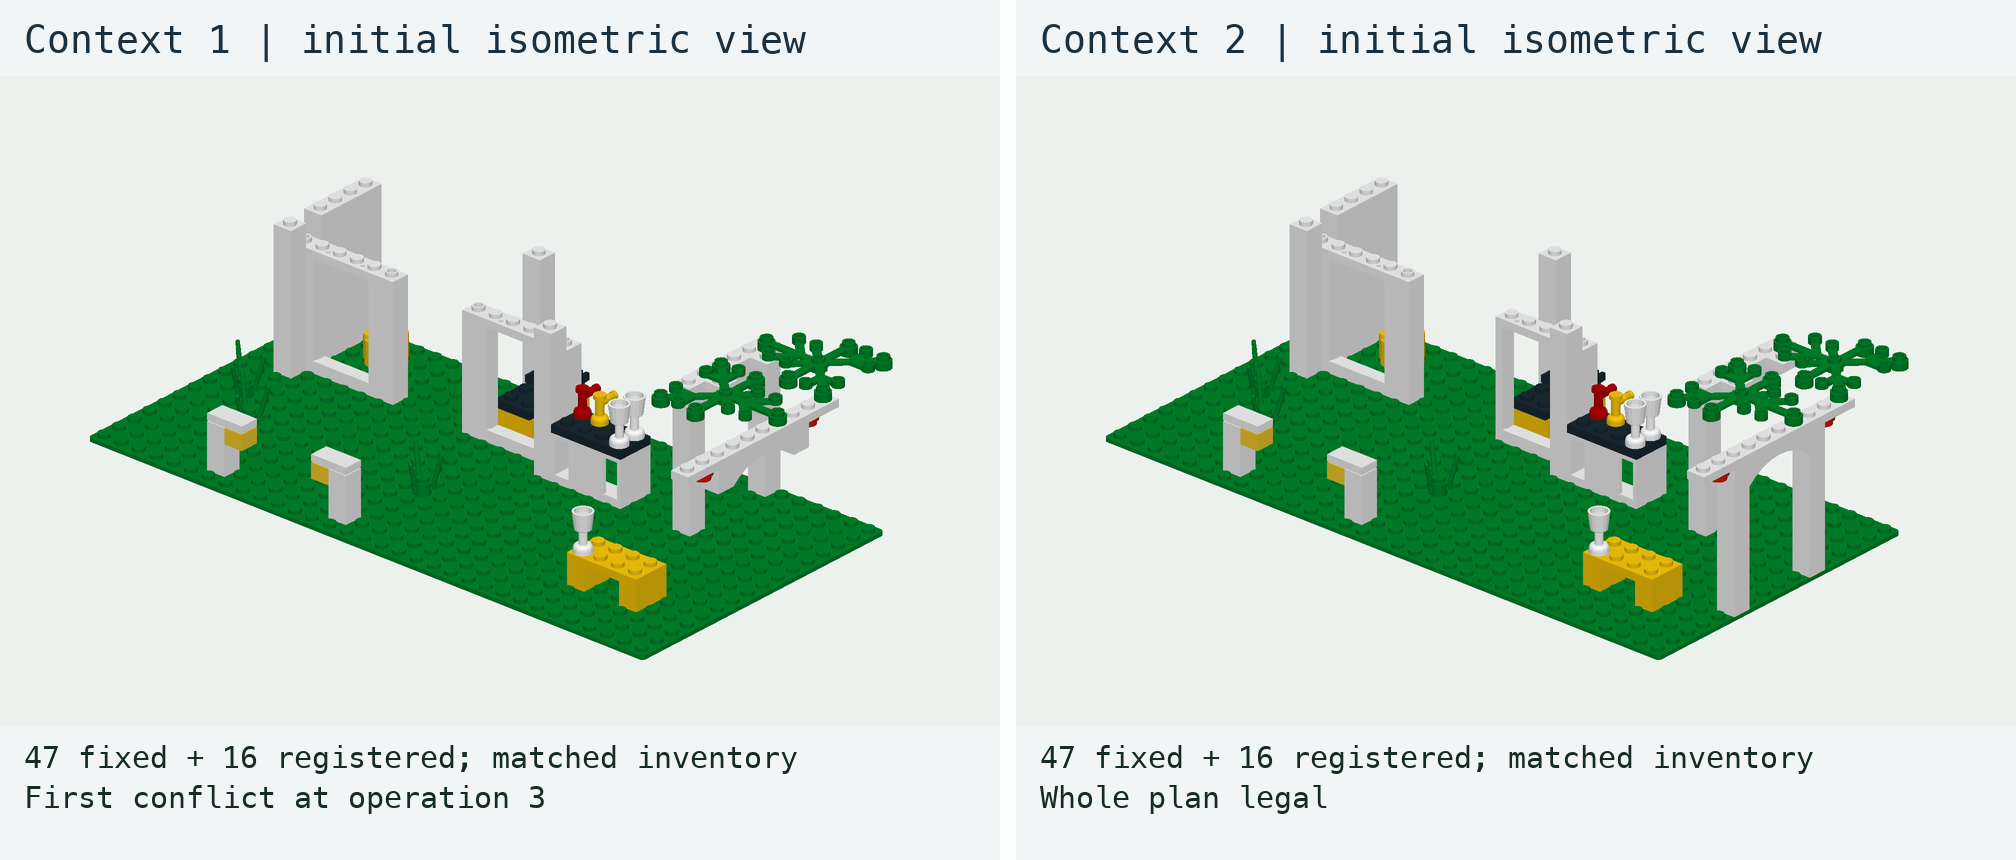
\includegraphics[width=.96\textwidth]{figures/geometry-contrast.png}
\caption{\GeometryCaseCaption}
\label{fig:geometry}
\end{figure*}

\section{Evaluation design}
\begin{table}[t]
\centering\small
\caption{Experiment framework. Population results are unmeasured;
model snapshots and provider settings must be fixed before collection.}
\begin{tabular}{p{.59\columnwidth}p{.30\columnwidth}}\toprule
Condition & Evidence status\\\midrule
Structural policies and exact search & Measured\\
SmolVLM-256M, image input & Historical failed case\\
Open / proprietary VLMs & Pending\\
Humans, images + registered IDs & Pending\\
Static / active / structured input & Matched study planned\\
Stepwise / explicit-plan prompting & Matched study planned\\
\bottomrule\end{tabular}
\label{tab:design}
\end{table}

Table~\ref{tab:design} fixes the reporting framework before empirical
collection. Primary episode outcomes are completion and optimal
completion over all assignments, plus excess operations among successes.
Diagnostic accuracy is reported by family, scoring role, canonical
problem, and source. Joint pair scores require both members correct.
Invalid outputs and missing assignments remain in their denominators.
Privileged structural policies are separate from image-input results.

The study compares matched assignments and identity seeds with declared
action and view budgets. For each VLM, static image and structured
conditions share the same initial views, executor, and answer syntax;
active acquisition is reported separately. A format/cost pilot precedes
the full study. Report snapshot, provider, prompt, image preprocessing,
context policy, decoding, calls, measured token use, and acquisition
count. Human collection requires documented instructions, training,
participant counts, and consent before recruitment.

Identity seeds, paired questions, and variants reuse source geometry.
Per-source results and coverage precede pooled claims.
\HeldoutSourceCount{} source groups are held out from development;
the primary geometry cohort covers \HeldoutPrimarySourceCount{} of them.
More diagnostic rows do not create more independent assemblies.
Errors are stratified into parsing, immediate legality, future cost,
diagnosis, and repair.

\section{Related work}
LTRON's Break and Make evaluates interactive structural understanding
through disassembly and reconstruction~\cite{ltron}. InstructioNet studies
construction supported by an agent's own explicit visual
instructions~\cite{instructionet}. These establish interactive brick
construction and long sequences; BrickPlan does not claim either as new.
Its registered-site action space permits exact counterfactual completion
costs and event-level recovery labels.

LEGO-Puzzles includes both elementary visual questions and a Planning
set~\cite{lego}; it should not be reduced to recognition.
PhyBlock combines hierarchical assembly and physical-understanding
questions~\cite{phyblock}. Brick-Composer introduces BC-Bench for diverse
brick selection and pose estimation~\cite{composer}. BrickPlan fixes
placement sites and instead measures resource coupling, future legality,
and delayed corridor return. It complements broader spatial tasks.

Shortest-path search and admissible heuristics are established
tools~\cite{astar}. Failure of a weak policy does not prove hardness.
We therefore include a strong static relaxation, capacity-aware dispatch,
bounded and full A*, and shallow-choice bounds. The contribution is
an auditable visual diagnostic instrument, not a new planning algorithm.

\section{Task and observation contract}
\subsection{State, geometry, and actions}
Let $A\subseteq V$ be occupied registered sites, $G\subseteq V$ the
target, $J\subseteq V$ required inspections, and $D\subseteq J$ completed
inspections. The mission state is $x=(A,D)$. Each piece $P_i$ belongs
to one original site $S_i$. Detached pieces occupy universal oversized
rack holders, subject to
\begin{equation}
 r(x)=|V\setminus A|\leq K.
\end{equation}
An \texttt{audit} completes a pending job only while its piece is detached;
completion persists after replacement. The terminal condition is
$A=G,\ D=J$, followed by an explicit \texttt{finish}.

An \texttt{attach} or \texttt{detach} must satisfy qualified straight
translation, collision, stud-connectivity, registration, and capacity
rules. Fixed pieces form a connected clamped assembly. Executable
positions preserve original LDraw transforms. Guarded inset meshes and
prescribed paths define qualification; this is not force, gravity, clutch,
hand-access, or arbitrary rigid-body simulation. Rack transfer is a
resource abstraction. Exploded views are reference diagrams, never
executable states.

Each physical operation or audit costs one operation; so does a rejected
operation attempt. Camera acquisition and diagnosis have separate budgets.
Episodes allow 12 additional views and 12 diagnoses. Public operation
budgets depend on visible problem size and work, not private optimum cost.

\subsection{Matched observations}
Five raster panels show the current assembly, target, all-site reference,
registered-piece catalog, and rack. Main views are supersampled at
$3840\times2880$ and reduced to native $1920\times1440$; catalog tiles
are $480\times360$. Text gives P/S registration, rack inventory, and the
inspection ledger. Image input omits pose matrices, installed-site flags,
legal-action lists, relation graphs, and exact costs. Explicit
registration simplifies correspondence without supplying geometric rules.

Static checkpoint diagnostics provide isometric, left, rear, and right
views at revision zero, with later acquisition disabled. Active image
diagnostics start with isometric only and charge one acquisition per
\texttt{inspect}. Structured diagnostics use the same four initial views
and additionally provide original matrices, colors, part types, path
directions and lengths, and occupancy. They omit the private
blocker/support graph; structural software controls receive that graph.
Interactive episodes retain their common active-view protocol.

Acquired frames persist with their revision. Free 3D orbit, explosion,
and answer review are available in unscored practice only. Human and
model policies share the controlled observation and submission contract.

\begin{table*}[t]
\centering\small
\caption{Seven public question families. Episode families are mutually
exclusive presentation groups. Every entry has an ID, prompt, constraints,
answer format, and scoring rule.}
\begin{tabular}{p{.20\textwidth}p{.39\textwidth}p{.31\textwidth}}\toprule
Family & Question & Response and measurement\\\midrule
Assembly / reconfiguration & Transform current assembly into target. & Actions; completion and excess cost\\
Finite-resource scheduling & Free the holders required for later work. & Actions under a capacity bound\\
Inspection / persistent state & Complete off-assembly work and restore target. & Actions and audits; physical and ledger completion\\
Next-action judgment & Which legal choice minimizes completion cost? & Index; any optimum accepted\\
Future-sequence checking & Where is the first illegal operation? & One-based index or \texttt{null}\\
Geometry / appearance & Does context change, or recoloring preserve, legality? & Conflict answer and joint pair score\\
Delayed error recovery & Which choice returns to the earlier optimal corridor? & Index on a shortest nonterminal repair\\
\bottomrule\end{tabular}
\label{tab:taxonomy}
\end{table*}

\subsection{Diagnostic formats}
Table~\ref{tab:taxonomy} separates interactive execution from checkpoint
questions. There are \NextActionCount{} next-action questions,
\ContinuationCount{} ordinary sequence questions,
\GeometryQuestionCount{} geometry questions,
\AppearanceQuestionCount{} appearance questions, and \RepairCount{}
delayed-repair questions. Sequence questions expose the complete proposed
plan and ask for its first illegal operation, or \texttt{null}.
Recovery questions expose the pre-error checkpoint, executed history,
current observation, and legal candidates. They ask for a shortest repair
step, not hidden model reasoning.

\section{Construction and validity controls}
\subsection{Source groups and sampling}
The \ProfileCount{} qualified geometry profiles include
\BaseProfileCount{} base assemblies and \ContextProfileCount{} context
profiles, including zero-yield candidates.
They belong to \SourceCount{} source kit groups. Alternate builds and
context variants remain within one group: roadster and kart both belong
to 31027. There are \DevelopmentEpisodeCount{} development episodes from
\DevelopmentSourceCount{} groups and \HeldoutEpisodeCount{} held-out
episodes from \HeldoutSourceCount{} disjoint groups.

Version 2.3 preserves the frozen 2.2 definitions and admits
\AdmittedCount{} of \CandidateCount{} new source candidates; all
\RejectedCount{} exclusions remain in the census. Candidate identities,
intake strata, source-group splits, and sampling are frozen before new
geometry qualification and solver discovery. Every newly admitted base
has at least eight registered and eight reachable movable sites.
Small historical domains remain regression cases, not new-source admissions.
An independent source audit subsequently excludes five candidates whose
part-only manifests omit direct model geometry and one with a conflicting
root kit identifier. Original files and preliminary admissions remain
archived; no replacement candidates are added. Every retained new-source instance
is bound to its exact original reference chain, identity, color and pose.

New-source geometry uses deterministic source-order collision pruning and
a bounded stud-connected component, preserving every retained original
instance and pose. Each admitted source supplies \GoalsPerSource{} goals,
\JobSettingsPerSource{} job settings, and \StartsPerMission{} starts per
mission: \NewSampledEpisodeCount{} seeded episodes in total. Solvability is
the only oracle-based admission condition; no policy score, cost gap, or
search effort selects these episodes. Legacy mechanism-conditioned tasks
and separately constructed geometry diagnostics retain explicit labels.
``New source'' does not mean absent from pretraining.

\begin{table}[t]
\centering\small
\caption{Fixed operation-length bins: D1 (1--8), D2 (9--16), D3
(17--24), D4 (25+). They are not cognitive-depth levels.}
\begin{tabular}{lrrrr}\toprule
Tier & Episodes & $C^*$ range & Gap range & A* max\\\midrule
D1 & 314 & 1--8 & 0--0 & 10\\
D2 & 701 & 9--16 & 0--4 & 311\\
D3 & 341 & 17--24 & 0--10 & 6,383\\
D4 & 65 & 25--42 & 0--18 & 14,307\\
\bottomrule\end{tabular}

\label{tab:tiers}
\end{table}

\subsection{Exact costs and difficulty descriptors}
For each mission, we enumerate the capacity-constrained physical
component and inspection-bit product. Reverse shortest paths give
$C^*(x)$, the minimum remaining operations. The \OracleCount{} tables
contain \ProductCount{} state entries and \EdgeCount{} directed-transition
entries, with physical states repeated under different goals and jobs.
Checks cover runtime transitions, physical inverses, lower bounds, and
Bellman equalities.

Let $R$ be occupied blocker closure needed to remove unwanted pieces,
insert target pieces, and detach unfinished inspection pieces. A static
relaxation is
\begin{equation}
 h(x)=|A\triangle G|+2|R\cap A\cap G|+|J\setminus D|.
\end{equation}
Each mismatch needs an operation, each occupied target piece in the
required closure needs removal and replacement, and each pending job
needs an audit. Capacity and connectivity can add operations. The maximum
retained gap $C^*-h$ is \MaxGap{}. Registered sites, rack size, occupancy,
jobs, gap, and search effort are separate descriptors; length bins alone
do not imply planning difficulty.

\subsection{Sequence and shallow-choice controls}
The \SequencePairCount{} legal/corrupted sequence pairs match first and last actions,
action multisets, and prefixes before the first conflict. Legal witnesses
contain no repeated-state padding. Each conflict bin (2--5, 6--10, 11+)
has \SequencePairsPerBin{} pairs. A prefix-only control executes $k$ operations and otherwise
answers ``all legal.'' It scores \PrefixTwoCorrect{}/\PrefixTwoTotal{} at $k=2$
and \PrefixFiveCorrect{}/\PrefixFiveTotal{} at $k=5$;
zero-step accuracy is \PrefixZeroAccuracy{}. This tests a specific shortcut without
establishing immunity to other ones.

At \DepthOneContainsOptimal{} of \NextActionCount{} next-action checkpoints,
the depth-one closure minimizer set includes an optimal choice.
Uniform tie selection yields \DepthOneUniform{}
expected accuracy; uniform selection among all candidates yields
\UniformCandidateAccuracy{}.
This strong result uses privileged structural relations. We disclose
tie sizes, optimistic and pessimistic accuracy, and the matched
image/structured comparison rather than infer required reasoning depth.

\subsection{Geometry and appearance}
The primary cohort contains \PrimaryPairCount{} answer-changing pairs,
\PrimaryInterventionCount{} interventions, and \PrimarySourceCount{} source
groups. Both contexts match total count and the exact part-number/color
multiset, registered instances and original poses, start, target, rack,
jobs, and proposed plan. Only subsets of original fixed instances change;
fixed connectivity, full-assembly support, meshes, and paths are separately
qualified. No unequal-inventory fallback is allowed.
All retained primary failures concern stud support; motion-blocker
relations match between contexts.

Of \QualifiedInterventionCount{} qualified matched interventions,
\ZeroYieldInterventionCount{} yield no retained future contrast under the
declared search. Geometry-only context selection precedes answer-change
testing. Retaining answer-changing plans is mechanism conditioning, not
representative source sampling. The supplement reports every source,
intake stratum, candidate stage, zero-yield intervention, and conflict bin.
The \HistoricalPairCount{} earlier unmatched pairs are historical
regressions and never enter the primary visual score.

Native certificates compare all five panels in four initial views.
Pixel distinction (Figure~\ref{fig:geometry}) does not establish perceptual
sufficiency or successful active acquisition. The
\AppearancePairCount{} original/grayscale pairs preserve geometry, state,
plan, and answer; they test appearance invariance, not independent structures.

\begin{figure*}[t]
\centering
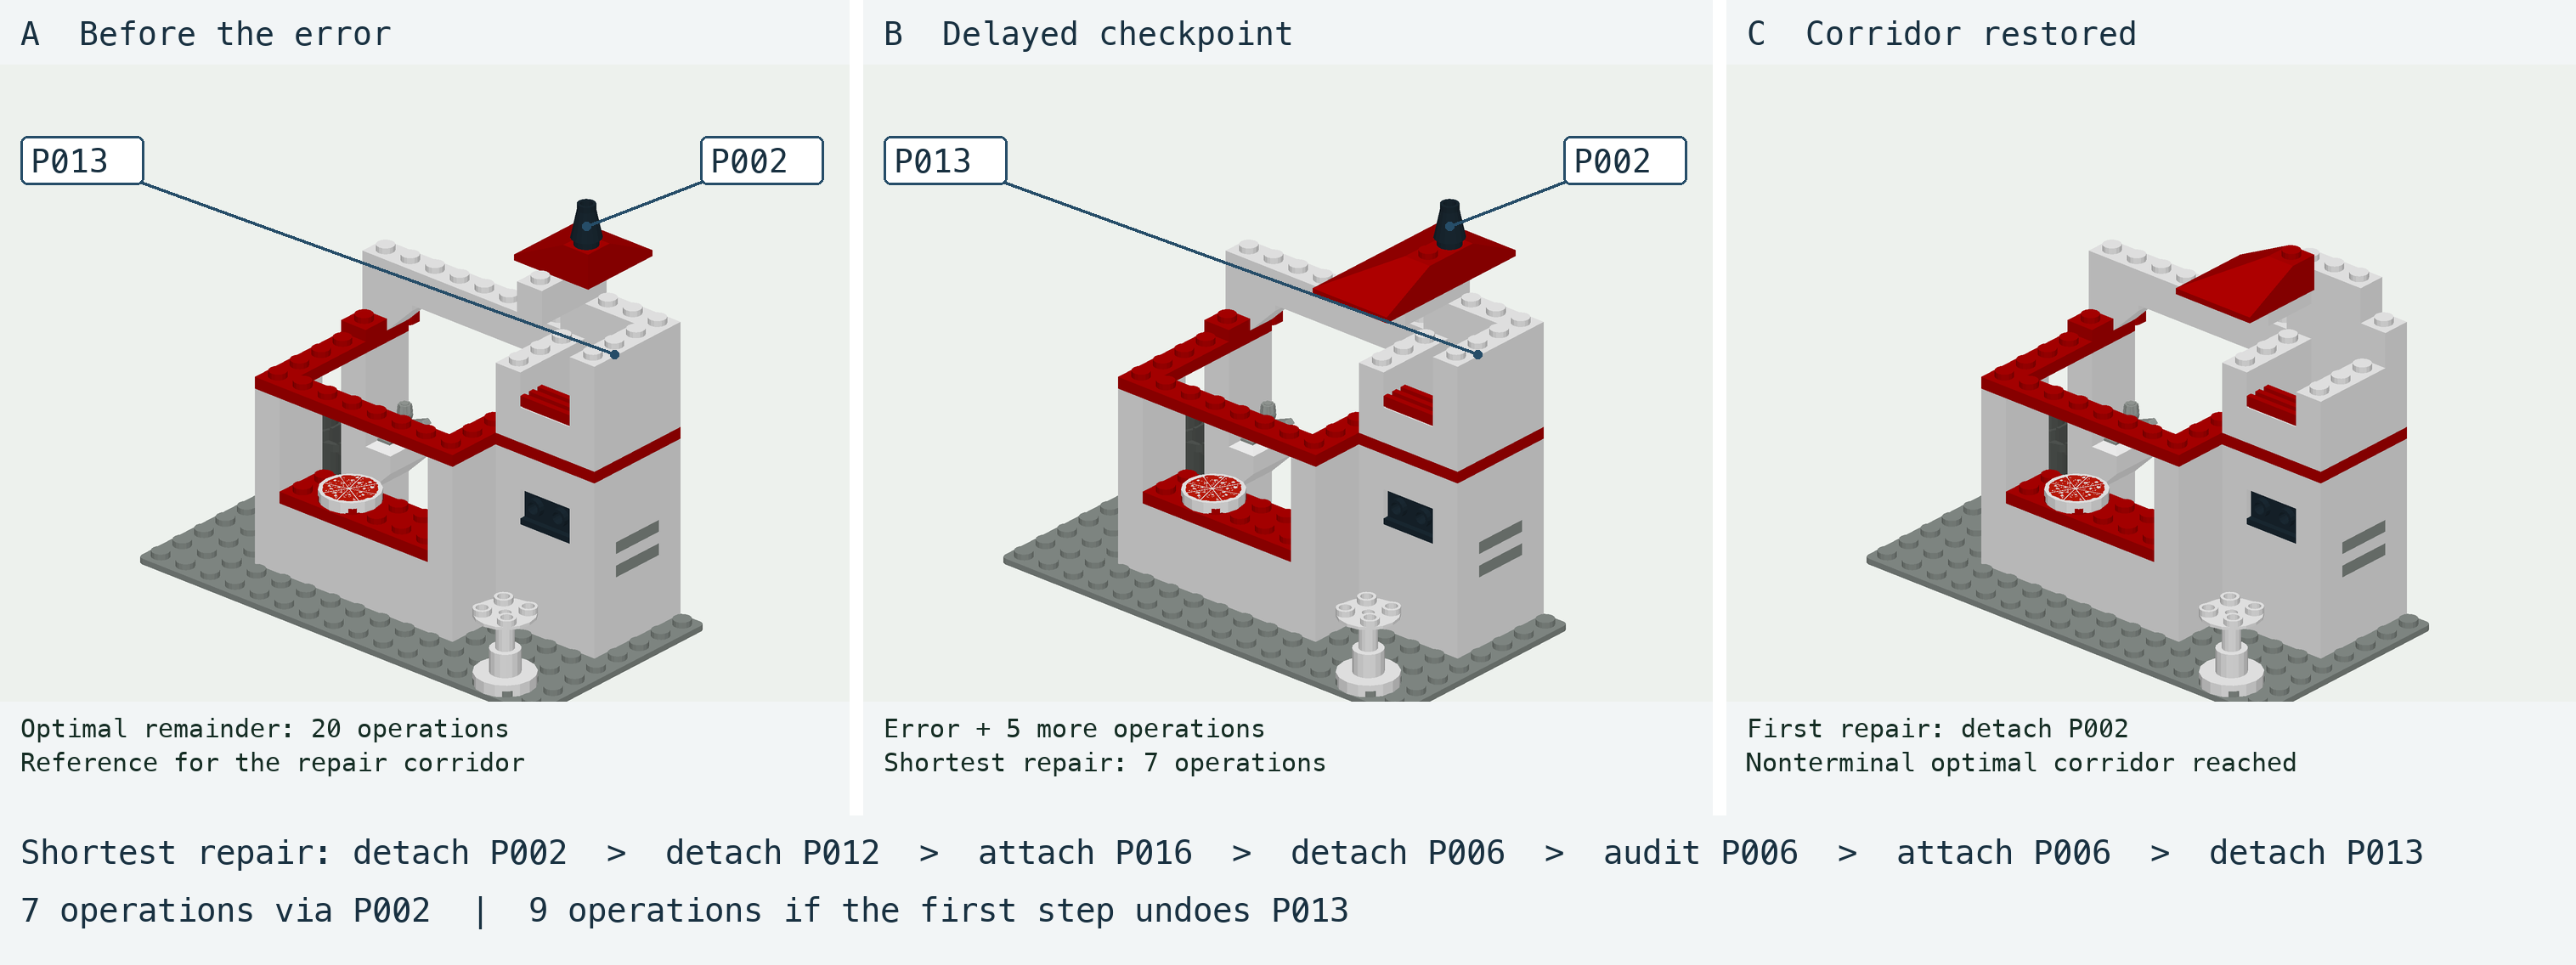
\includegraphics[width=\textwidth]{figures/repair-case.png}
\caption{\RepairCaseCaption}
\label{fig:repair}
\end{figure*}

\subsection{Delayed repair and calibration}
For a pre-error checkpoint $b$, let $\mathcal C_b^{-}$ contain all
nonterminal states on any optimal completion from $b$. After a legal
positive-excess error, a distinct-state legal history of lag 1, 3, or 5
remains outside this corridor. At checkpoint $z$, the repair target is
\begin{equation}
 r_b(z)=\min_{y\in\mathcal C_b^{-}}\operatorname{dist}(z,y).
\end{equation}
The \RepairCount{} questions have repair costs \RepairMin{}--\RepairMax{}, independently verified by
forward BFS. Any first action on a shortest repair is accepted.
Finishing after a costly detour does not itself earn repair credit.

Lag alone does not establish nonlocal repair. Reversing the last public
action solves \InverseCorrect{}/\RepairCount{} questions (\InverseAccuracy{});
the inverse is suboptimal on \InverseSuboptimal{} and unavailable on
\InverseUnavailable{}. These cohorts are reported separately.
All \CalibrationCount{} questions with every candidate optimal remain
calibration checks and receive no weight in discriminative accuracy.

\section{Metrics and scoring units}
For a legal unit-cost action with successor $x'$, conditional excess is
\begin{equation}
 \delta(x,a)=1+C^*(x')-C^*(x)\geq0.
\end{equation}
A rejected attempt leaves state unchanged and contributes one excess
operation. Thus legal but costly actions remain distinct from immediate
invalidity even when rework was already mandatory. Successful regret
is $T-C^*(x_0)$ for $T$ charged attempts. Completion and optimal completion
use all assignments; mean successful regret accompanies its coverage.

Every legal positive-excess action opens a recovery event. Later errors
do not overwrite earlier events. Restoration, immediate and lag-specific
cohorts, and right-censored unfinished trajectories are recorded
separately. Diagnosis concerns avoidable errors since the last diagnosis;
mandatory rework is not an error. Suffix effort is compared with exact
remaining cost at diagnosis. Survival curves preserve the first cost-loss
event after later recovery, with assigned and unknown counts at each step.
The reversible physical components and persistent audits contain no
genuine irreversible dead ends; their eligible-choice rate is undefined.

The \ProbeCount{} rows represent \ProblemCount{} canonical diagnostic
problems; repeated statements and appearance variants account for
\RepeatedRowCount{} excess rows. Canonical identity includes source geometry, state,
target, work, capacity, and the exact question or history.
There are \DiscriminativeCount{} discriminative assignments.
Primary accuracy averages assigned variants within a canonical problem,
then problems within a source, then sources equally. Missing variants
receive zero before averaging. Row, problem-macro, source-macro,
calibration, and recovery-cohort scores remain available. Primary geometry
correctness requires \emph{both exact first-conflict labels}, not merely
a predicted answer change. Any assigned member makes a pair eligible;
a missing partner, absent response, or malformed label earns zero joint
credit. Wholly unassigned pairs remain census-only. Repeated rows are
averaged within distinct starts, then interventions, then sources.
Whole-source bootstrap intervals and leave-one-source-out summaries
describe sensitivity conditional on retained sources, not population coverage.
The supplement details metric denominators and regret conservation.

\section{Measured evidence}
\begin{table*}[t]
\centering\small
\caption{Structural controls on \EpisodeCount{} episodes. The oracle
uses one seed; other policies use three tie-order seeds (\PolicyRuns{}
runs). Regret is mean excess among successes. Exact relations are
privileged inputs, so these are not image-input VLM results.}
\begin{tabular}{lrrrrr}\toprule
Control & Runs & Success & Optimal & Regret & Max exp.\\\midrule
Exact oracle & 1421 & 1421 & 1421 & 0.00 & ---\\
Closure greedy & 4263 & 4163 & 3642 & 1.77 & ---\\
Capacity dispatch & 4263 & 4132 & 3642 & 1.80 & ---\\
Closure A* (100) & 4263 & 4075 & 4075 & 0.00 & 100\\
Closure A* (1,000) & 4263 & 4199 & 4199 & 0.00 & 1,000\\
Closure A* (full) & 4263 & 4263 & 4263 & 0.00 & 14,307\\
Hamming A* (full) & 4263 & 4263 & 4263 & 0.00 & 230,679\\
Legal random & 4263 & 265 & 60 & 13.11 & ---\\
Drop inspections & 4263 & 1536 & 1536 & 0.00 & ---\\
Ignore rack limit & 4263 & 3595 & 3595 & 0.00 & ---\\
\bottomrule\end{tabular}

\label{tab:controls}
\end{table*}

\subsection{Structural policies}
Closure greedy minimizes the static successor bound with visited-state
and randomized site tie-breaking. Capacity dispatch prioritizes audits,
mandatory removals, safe placements, and temporary staging, with
revisited-state escape. Greedy completes \GreedyCompleted{}/\GreedyAssigned{}
runs, with \GreedyOptimal{} optimal; dispatch completes
\DispatchCompleted{}/\DispatchAssigned{}, with \DispatchOptimal{} optimal.
Completion alone
therefore conceals avoidable effort (Table~\ref{tab:controls}).

A* uses graph reopening, $(g+h,h)$ priority, and declared limits without
oracle access. Limits of 100 and 1,000 expansions complete
\BoundedSmallCompleted{} and \BoundedLargeCompleted{} runs.
Full closure A* completes \FullSearchCompleted{}/\FullSearchAssigned{},
\FullSearchOptimal{} optimally, with median \FullSearchMedianExpansions{}
and maximum \FullSearchMaxExpansions{} expansions.
The weaker occupancy-plus-pending-audit
heuristic is also reported. These perfect-information measurements
constrain difficulty claims; weak controls alone can inflate them.

Dropping inspection obligations or ignoring rack limits produces
failures when relaxed plans execute under the actual rules. These are
model-mismatch ablations, not strong planners. Raw actions, states,
rejections, expansions, timings, and every aggregate are released.
Seeds repeat geometry and tie order; cached local timings are not
calibrated cross-platform comparisons.

\subsection{Reduced-input geometry controls}
\begin{table*}[t]
\centering\small
\caption{Primary inventory-matched geometry: deterministic software rules,
not visual performance. Joint correctness requires both exact labels.
Intervals resample whole source groups; unavailable estimates are marked
unavailable, never inferred as zero.}
\begin{tabular}{llrrrrl}\toprule
Software rule & Split & Pairs & Sources & \shortstack{Joint\\micro} & \shortstack{Source\\macro} & \shortstack{95\%\\interval}\\\midrule
Named-occupancy inventory & Dev. & 12 & 3 & 0.0\% & 0.0\% & [0.0, 0.0]\\
Named-occupancy inventory & Held out & 24 & 9 & 0.0\% & 0.0\% & [0.0, 0.0]\\
Public-text inventory & Dev. & 12 & 3 & 0.0\% & 0.0\% & [0.0, 0.0]\\
Public-text inventory & Held out & 24 & 9 & 0.0\% & 0.0\% & [0.0, 0.0]\\
Development source majority & Held out & 24 & 9 & 0.0\% & 0.0\% & [0.0, 0.0]\\
\bottomrule\end{tabular}

\label{tab:shortcuts}
\end{table*}
Count-only, type/color-presence, type/color-count, and sequence-only
certificates test explicitly restricted representations. Equal inputs with
unequal labels cannot both be correct for a deterministic single-member
function of that representation. These label-aware finite-bank ceilings
are not fitted held-out predictors, and do not cover instance-sensitive
spatial reasoning or policies using pair position as extra information.
Separate label-free inventory execution rules and a source-majority
predictor fitted only on development labels appear in
Table~\ref{tab:shortcuts}. Exact inventories and named occupancy are
privileged perception abstractions, not measured visual extraction.

\subsection{Historical model integration case}
The workbench preserves a version-2.1 SmolVLM-256M-Instruct run on
\texttt{kart-deck-08} (historical public E069, seed 0). All four calls
return scene descriptions instead of JSON actions. Each becomes
\texttt{INVALID\_ACTION}, consumes an operation, and leaves the state
unchanged. The controller stops at four calls. This is a failed
integration example, not a planning or population result.

The original task, bank hash, image bytes, prompts, raw outputs, parsed
actions, feedback, latency, measured MLX token counts, and weight digest
are preserved. Native stimuli are 1920 pixels wide; this model's processor
resizes the longest edge to 512 with splitting disabled. HD display does
not imply native-HD inference. Historical E069 is not relabeled as a
version-2.3 experiment. An OpenAI-compatible practice adapter and a
separate usage-accounted study runner support further collection.

\section{Release and limitations}
The React workbench exposes seven families, complete previews, ID/source/
split filters, answer submission, model playback, and review-JSON export.
Its isolated WebGL2 renderer preserves original geometry, supports free
practice orbit and explosion, and shows part details on hover.
Native zoom preserves raster evidence. Dataset cards, public JSONL,
sample HD inputs, evaluator dependencies, and deployment files are
packaged together. No external hosting URL is claimed.

Software validation replays all \EpisodeCount{} optimal episodes and
\ProbeCount{} answers. Audits check sequence multisets, source separation,
repair BFS labels, input-pixel differences, budget accounting, missing
assignments, overlapping errors, and transcript tampering. Protocol and
browser checks cover persistence, observation isolation, and playback.
This establishes software behavior, not human usability or real-world
mechanical validity.

The principal limits remain structural and empirical. Perfect-information
controls characterize this finite bank, not visual planning competence.
Registration and inventories simplify grounding. Matched inventories remove
the former global-count confound, not every instance-level spatial shortcut.
Pixel distinction still needs empirical answerability testing.
Geometry excludes forces, arbitrary poses, rotations,
simultaneous subassembly motion, and real rack transfers. Source scale
does not eliminate dependence, admission bias, or public-CAD contamination.
No model shortsightedness,
human--model gap, or immunity to all shortcuts has been measured.
The next study must report matched static, active, and structured inputs,
source-level uncertainty, and coverage across retained context interventions.

\newpage
{\small
\bibliographystyle{ieeenat_fullname}
\bibliography{references}
}
\end{document}
